\begin{apendicesenv}

\partapendices

\chapter{Termo de Abertura do Projeto}

\subsection{Objetivos deste documento}

Mesmo já havendo um consenso de ideia geral sobre o projeto, o TAP vem para autorizar formalmente o seu desenvolvimento, seja para as fases seguintes de planejamento, seja para construção efetiva da proposta. Ele também auxilia na definição de entregas por meio da EAP, no levantamento de requisitos, premissas e restrições, além de dar o grande suporte para o resto do planejamento, custo, riscos, tempo, escopo etc.

Elaborado este documento, o gerente de projetos tem a autorização, o poder e a base para o gerenciar corretamente todos os recursos disponíveis e otimizar seu planejamento durante o desenvolvimento do produto. Não deve ser esquecido que este documento deve ser descrito de forma que forneça suporte suficiente na aceitação ou não do projeto.


\subsection{Descrição do Projeto}

O projeto é uma máquina automática que auxilia no processo de reciclagem de garrafas. A ideia central é a de que o usuário insira garrafas de vidro ou plástico e seja bonificado por essa ação, onde tal, possa ser desconto em supermecados e estes dados serão mantidos por um aplicativo com contas individuais. A máquina deverá realizar a separação e validação (material, tamanho e peso) automática dos objetos inseridos, guardando a garrfas de vidro sem quebrá-las, triturando as de plástico e rejeitando qualquer outro tipo de inserção.

\subsection{Justificativa do Projeto}

A poluição global é um tema que visivelmente está sempre em discussão na mídia e nos governos por seu grande potência destrutivo. Dois dos grandes tipos de poluição que podem ser comentadas neste projeto são as de solo e do mar, sendo o motivo desta escolha comentado mais a frente, e é evidente que se sabe que o causador dessa agressão a esses dois tipos é o grande volume de material industrial criado pelo ser humano. Buscando minimizar esse problema, são realizadas diversas ações de reciclagem e conscientização ao redor do globo, sendo assim, este projeto vem com o intuito de criar um produto que motive estes dois fatores.

Para o desenvolvimento de um protótipo foram escolhidos dois tipos de materiais a serem coletados a partir das informações a seguir. O primeiro foi o plástico, pois segundo o site \cite{ecycle}, pesquisadores da The University of  Western Australia e da CSIRO Wealth from Oceans Flagship realizaram um estudo no mar australiano e concluíram que a cada quilômetro quadrado de água de sua superfície está contaminado por cerca de quatro mil pequenos fragmentos de plástico. Segundo o site da Globo \cite{oglobo}, até 2015 tinham sido produzidos cerca de 6,3 bilhões de toneladas de resíduos plásticos e 79\% deste montante se encontra em aterros ou na natureza. Segundo o site \cite{culturamix}, sacolas plásticas e garrafas PETs são os maiores vilões da natureza pelo tempo de decomposição e pelo consumo destes materiais por animais. E o segundo foi o vidro pelo alto consumo de produtos mantidas em recipientes feitos deste material, o vidro pode causar queimadas na natureza por potencializar os raios solares e animais podem morrer ao ingerir pedaços cortantes. Portanto, serão dois materiais que causarão um grande impacto de projeto e eles estão diretamente ligados às poluições marítimas e de solo.

Outro fator que justifica a proposta deste projeto, são os impactos positivos para os usuários, que poderão receber créditos pela sua ação, empresas de reciclagem, que terão economia de armazenamento e manuseio, o governo, que terá seu nome em um projeto de apoio ambiental, os mercados, que poderão atrair mais clientes com promoções por conta da máquina e empresas geradoras dos resíduos já que pela lei nacional, elas são responsáveis pelo seus resíduos sólidos.

\subsection{Objetivos do Projeto}

O máquina tem como objetivos principais o incetivo a reciclagem por meio de um sistema de bonificações, o auxílio a coleta de material para as empresas de reciclagem e auxílio às empresas geradoras de resíduos sólidos já que elas são responsáveis pelo o que produz.

\subsection{Critérios de sucesso do projeto}

Tomando como referência o contexto de implantação do produto, os critérios de sucesso do projeto envolvem a dedicação máxima e estudo contínuo da equipe em seus subsistemas já que em sua maioria não se há investimento e nem experiência de trabalho. Rigorosa adesão ao planejamento e gerenciamento do projeto. Alcance dos requisitos levantados e integração completa.

\subsection{Estrutura Analítica do Projeto}

\begin{figure}[!ht]
	\centering
		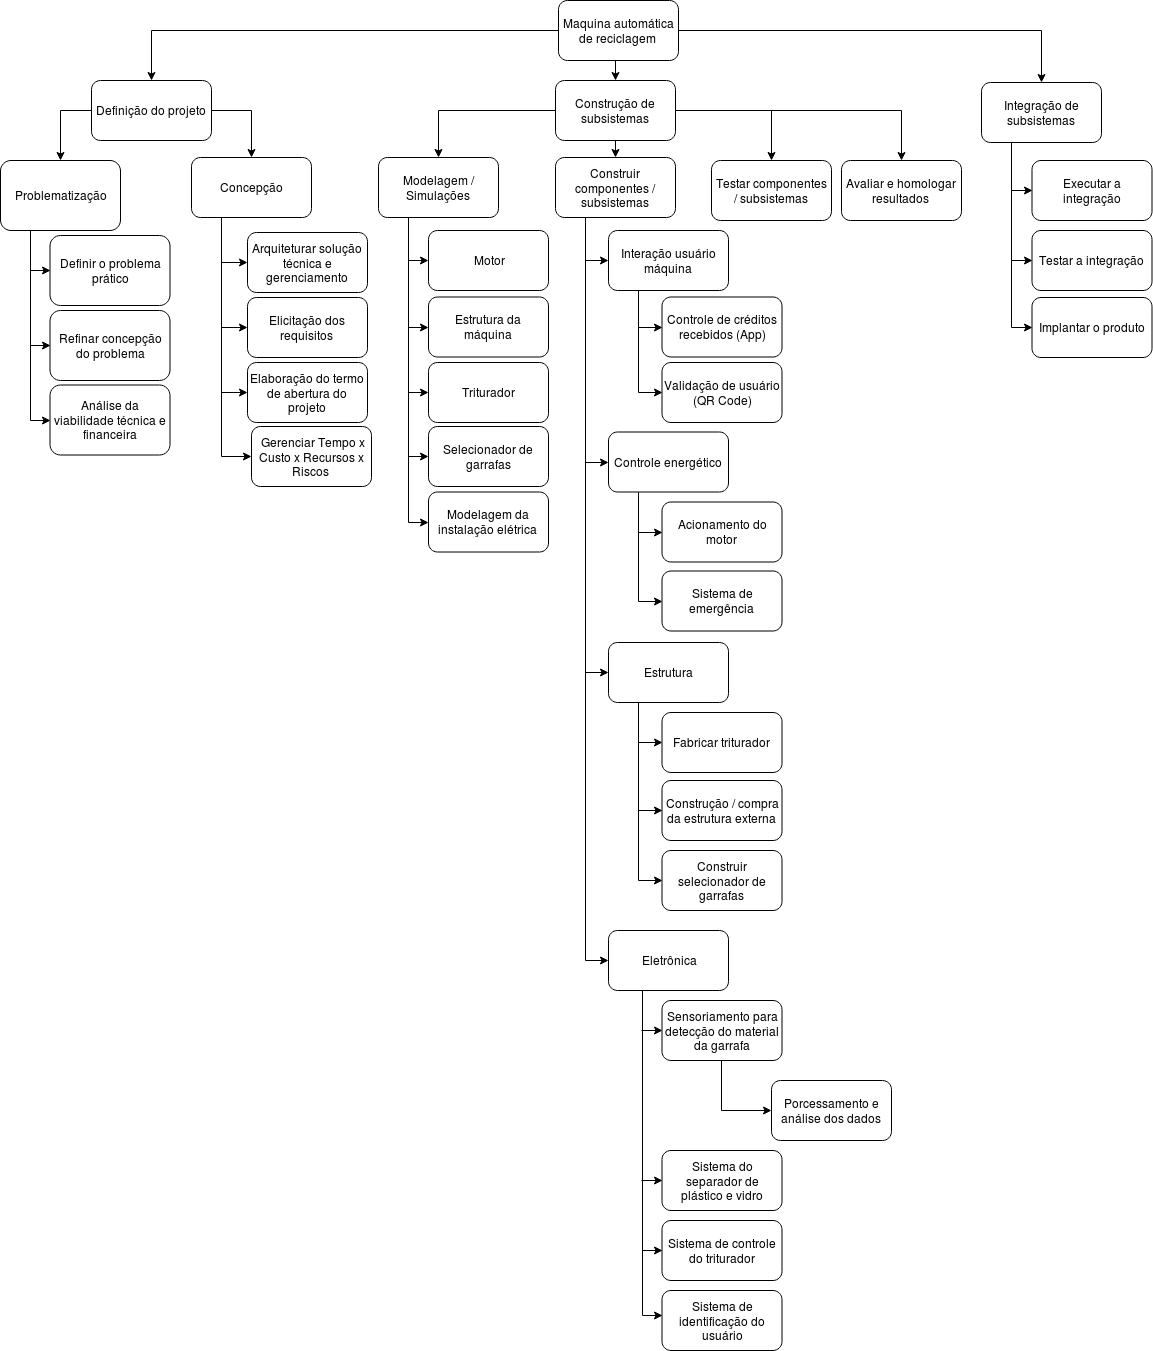
\includegraphics[scale=0.4]{figuras/eap}
	\caption{Estrutua Analítica do Projeto.}
\end{figure}

A EAP deste projeto está divida com base nas entregas definidas pelos orientadores. Como em todo projeto que se preze, o desenvolvimento do produto se sustenta na definição de um problema, elaboração de uma solução, construção do produto da solução e implantação e teste deste produto, logo abaixo estão descritos cada tópico da estrutura analítica voltados às necessidades de acompanhamento e gerência dos subsistemas deste projeto.

\begin{itemize}
    \item \textbf{Definição do projeto}
        Todo novo desenvolvimento de produto se inicia com a definição completa e planejada de um escopo geral e validado. Para começar, de forma geral, não seria viável a elaboração de um produto que não se resolve nenhum problema, sendo assim, é interessante a fase de definição ser divida na \textbf{Problematização} e \textbf{Concepção} baseada no ideia levantada.
        \begin{itemize}
            \item \textbf{Problematização}
                Essa fase envolve a aplicação de brainstormings para que o grupo possa avaliar o que há de problemas baseados na ideia central de projeto, para que assim, sejam anotados de forma planejada alguma de suas soluções que estejam ao alcance às áreas de conhecimento dos cursos da FGA. Em seguida, o problema deve ser refinado, de forma, que forneça base para a concepção completa e compreensível do escopo geral do produto que no caso é a solução proposta e para a análise da viabilidade técnica e financeira.
            \item \textbf{Concepção}
                Tendo sido levantada a ideia geral do projeto, aqui devem ser feitas os detalhamentos da arquitetura básica da solução, dos objetivos, regras de negócio e planejamento.
        \end{itemize}
    
    \item \textbf{Construção de Subsistemas}
        Após concretizado a definição do projeto, é o momento de iniciar o processo de desenvolvimento da máquina. Procurando facilitar a visão geral e organização, este processo foi divido em 4 atividades chaves:
        \begin{itemize}
            \item \textbf{Modelagem / Simulações}
                Uso do CAD, realização de cálculos diversos, uso de ferramentas de modelagem e geração de modelos de protótipos.
            \item \textbf{Construir componentes / Subsistemas}
                O sistema total do projeto foi dividido em 4 subsistemas com base nas áreas das engenharias com o intuito de otimizar a produtividade desacoplando as áreas. Nesta fase que acontece a construção real da máquina.
            \item \textbf{Testar componentes / Subsistemas}
                Fase de aplicação de plano de testes do componentes dentro dos subsistemas.
            \item \textbf{Avaliar e homologar resultados}
                Finalizado os testes, este é o momento de avaliar os resultados para levantamento do que deve ser otimizado afim de adaptar os componentes à atividade de integração. 
        \end{itemize}

    \item \textbf{Integração de Subsistemas}
        Esta em tese é a atividade mais complexa e que se tem um histórico alto de falhas, sendo assim, é necessário uma ótima preparação antecipada.
\end{itemize}

\subsection{Requisitos}
\subsubsection{Requisitos de Alto Nível}
O sistema proposta será um máquina com sua estrutura do tamanho de uma geladeira pequena no formato retangular, a estrutura interna será dividida em acordo com os subsistemas do produto total. Haverão dois compartimentos removíveis, um para o armazenamento de plástico triturado e outro para armazenar vidro, sendo os materiais aceitos pela máquina apenas como garrafas. Contando que o plástico será guardado em pedaços triturados, deverá haver um triturador que será ligado a partir de um motor em conjunto com um redutor. Já o vidro deverá ser armazenado intacto pilhando as garrafas.

Para armazenar algo, deve-se ter a devida validação daquilo que for aceito como armazenável ou não, e também deve-se ter uma estrutura de separação de materiais que os conduzam por estruturas diferentes, para que assim, atenda os cuidados requeridos que inferem aos requisitos necessários a cada material. Sendo assim, logo na frente da máquina, terá a validação do objeto inserido por meio de um QR Code que virá contido no rótulo, logo no bocal de inserção haverá uma outra validação mais completa em que passada dela, a garrafa será direcionada ao ponto final de armazenamento.

A máquina deverá ter um sistema de recompensa ao usuário por cada garrafa depositada, onde essa atividade será administrada por meio de um aplicativo. Haverá um banco de dados com as características de cada rótulo identificado para validação de entrada e de pontuação. Por fim terá um sistema de segurança de parada do motor.

\subsubsection{Principais requisitos das principais entregas/produtos}

\begin{itemize}
    \item{Armazenamento de garrafas de plástico e vidro}
    \item{Armazenamento separado dos tipos de material}
    \item{Triturar as garrafas de plástico}
    \item{Armazenar em intacta as garrafas de vidro}
    \item{Bonificar os usuários por cada garrafa}
    \item{Manter dados do usuário em um aplicativo}
\end{itemize}

\subsection{Marcos}

\begin{table}[htp]
    \centering
    \caption{Marcos}
    \label{my-label}
    \begin{tabular}{|p{0.25\linewidth}|p{0.65\linewidth}|p{0.15\linewidth}|}
    \hline
    \multicolumn{1}{|c|}{\textbf{Fase}} & \multicolumn{1}{c|}{\textbf{Marcos}} & \multicolumn{1}{c|}{\textbf{Previsão}} \\ \hline
    Iniciação & Projeto Aprovado & 28/03/2018 \\ \hline
    Planejamento & Plano de Gerenciamento de Projetos Aprovado & 28/03/2018 \\ \hline
     & Linhas de Base de Custos, Prazo e Escopos Salvas & 28/03/2018 \\ \hline
    Execução, Monitoramento e Controle & Desenvolvimento dos subsistemas & 16/05/2018 \\ \hline
    Encerramento & Integração & 26/05/2018 \\ \hline
     & Testes & 06/06/2018 \\ \hline
     & Projeto Entregue & 22/06/2018 \\ \hline
    \end{tabular}
\end{table}

\subsection{Partes interessadas do projeto}

É preferível pela equipe de trabalho que as partes interessadas sejam divididas em dois grupos, o primeiro são os reais interessados dentro do contexto e escopo atual que é a matéria do curso, e o segundo são os possíveis interessados em uma possível implantação comercial deste produto.

\subsubsection{Partes interessadas em cenário acadêmico}

\begin{table}[htp]
    \centering
    \caption{Cenário acadêmico}
    \label{my-label}
    \begin{tabular}{|p{0.30\linewidth}|p{0.30\linewidth}|p{0.30\linewidth}|}
    \hline
    \multicolumn{1}{|c|}{\textbf{Nome}} & \multicolumn{1}{c|}{\textbf{Função}} & \multicolumn{1}{c|}{\textbf{Interesse}} \\ \hline
    Professores da Matéria Projeto Integrador II do Campus de Engenharias da UnB & Orientar e avaliar os alunos no desenvolvimento do projeto & Orientar e avaliar os alunos no desenvolvimento do projetoSaber se os alunos da matéria estão hábeis a serem egressos da universidade \\ \hline
    Alunos da Matéria Projeto Integrador II do Campus de Engenharias da UnB & Desenvolver o projeto & Receber feedback da qualidade do projeto e da qualidade de trabalho. \\ \hline
    \end{tabular}
\end{table}

\subsubsection{Partes interessadas em cenário de mercado}

\begin{table}[htp]
    \centering
    \caption{Cenário de mercado}
    \label{my-label}
    \begin{tabular}{|p{0.30\linewidth}|p{0.30\linewidth}|p{0.30\linewidth}|}
    \hline
    \multicolumn{1}{|c|}{\textbf{Nome}} & \multicolumn{1}{c|}{\textbf{Função}} & \multicolumn{1}{c|}{\textbf{Interesse}} \\ \hline
    Clientes de supermercado & Utilizar a máquina & Ser bonificado pelo uso \\ \hline
    Empresas de reciclagem & Buscar e reciclar o material armazenado pela máquina & Economizar em manuseio e transporte do material \\ \hline
    Empresas geradoras de Resíduos Sólidos & Gerar os resíduos sólidos & Economia na gerência de seus resíduos \\ \hline
    Governo & Aplicar e apoiar serviços deste cunho & Ter um projeto deste cunho vinculado ao seu nome \\ \hline
    \end{tabular}
\end{table}

\subsubsection{Restrições}
O projeto está restrito a ser um protótipo por conta do tempo de projeto (um semestre letivo), inexperiência da equipe (primeiro experiência de projeto em conjunto com o intuito de integração de várias áreas de engenharia) e falta de orçamento (máximo de R\$ 3.900,00).

\subsubsection{Premissas}
\begin{itemize}
    \item{Os testes de uso serão realizados apenas com os integrantes do time de desenvolvimento}
    \item{O tempo de trituração poderá ser avaliado apenas durante o desenvolvimento}
    \item{A prova de integração entre o aplicativo e a máquina será via display simples}
    \item{A disponibilidade de horário comum da equipe é apenas no horário de aula}
    \item{Não haverá recursos vindos de fora da equipe}
\end{itemize}

\subsubsection{Riscos}
Os principais riscos levantados inicialmente são:
\begin{itemize}
    \item{Inexperiência dos membros da equipe com ferramentas e tecnologias a serem utilizadas}
    \item{Peças que demoram a ser obtidas estarem com defeito}
    \item{Aceito não gratuito a equipamentos de alto curto realmente necessários}
    \item{Falta de espaço para construção da estrutura}
    \item{Falha na integração}
\end{itemize}

\subsubsection{Orçamento do Projeto}
\begin{table}[htp]
    \centering
    \caption{Orçamento}
    \label{orcamento}
    \begin{tabular}{|l|l|}
    \hline
    Ambiente do Usuário & R\$ 00,00 \\ \hline
    Sistema de Controle de Energia e Segurança & R\$ 1370,00 \\ \hline
    Estrutura & R\$ - \\ \hline
    Sistema Eletrônico & R\$ 520,00 \\ \hline
    \multicolumn{2}{|c|}{\textbf{R\$ 1.890,00}} \\ \hline
    \end{tabular}
\end{table}
    

\chapter{Plano de Gerenciamento de Riscos}

\subsection{Introdução}
O propósito deste documento é identificar e mapear os riscos em busca de controlá-los e assim, minimizar fortemente os percentuais de falhas e possíveis fracassos em relação a gestão e desenvolvimento.

\subsection{Metodologia}
A metodologia para o gerenciamento dos riscos será baseada no modelo espiral definido por Boehm em 2004, onde a cada ciclo da espiral, é feito uma análise de riscos para validação. Neste projeto, será feito uma adaptação do modelo, as análises serão realizadas ao final de cada sprint.

As ferramentas que serão utilizadas para a gerência dos riscos seguem uma ordem de apoio bem sincronizada, a primeira é o What if, que “é uma técnica qualitativa de cunho geral, de simples aplicação e muito útil como primeira abordagem na identificação e detecção de riscos, em qualquer fase do projeto ou processo.” \cite{blogtek}, esta técnica será usada ao início de cada sprint e quando a equipe ver a necessidade e seus resultados serão guardados no registro de riscos. Método de utilização:
Construir a seguinte tabela em grupo pensando nas atividades mais influenciadoras para sequência do projeto:

\begin{table}[htp]
    \centering
    \caption{WhatIf}
    \label{my-label}
    \begin{tabular}{|l|l|l|l|l|}
    \hline
    \multicolumn{1}{|c|}{\textbf{Atividade}} & \multicolumn{1}{c|}{\textbf{O que aconteceria se ?}} & \multicolumn{1}{c|}{\textbf{Causas}} & \textbf{Consequências} & \textbf{Observações} \\ \hline
     &  &  &  &  \\ \hline
    \end{tabular}
\end{table}

A segunda é o Checklist, onde “trata-se de uma ferramenta de contribuição, uma vez que precisa que os riscos já tenham sido identificados anteriormente em outros processos. Serve para verificar a aplicação das medidas recomendadas em processos de análise de risco anteriores. ”\cite{qualidadesimples}, ou seja, é uma ótima técnica para complementar o levantamento e monitoramento de aplicações de medidas contra os riscos. Método de uso do checklist:

Após identificado os riscos, usando o What If e o registro dos riscos, deve-se elaborar uma lista com checklists verificando se as respostas ao riscos encontrados surtiram efeito. Então as ações de sucesso ficam guardadas. Exemplo:

\begin{table}[htp]
    \centering
    \caption{Checklist}
    \label{my-label}
    \begin{tabular}{|l|l|l|l|}
    \hline
    \multicolumn{1}{|c|}{\textbf{Risco}} & \multicolumn{1}{c|}{\textbf{Solução}} & \multicolumn{1}{c|}{\textbf{Resposta}} & \multicolumn{1}{c|}{\textbf{Observações}} \\ \hline
     &  &  &  \\ \hline
    \end{tabular}
\end{table}

\subsection{Processo de Gerência de Riscos}
É definido, ainda no PMBOK, como será realizada a gerência, ou seja, a sequência de atividades que possibilitará o monitoramento dos riscos. Abaixo se encontra um diagrama que demonstra o processo que envolve este plano e logo em seguida é explicado cada etapa e sua associação com as ferramentas e fontes de dados escolhidos. O planejamento da gerência não é listado, pois já está fazendo parte da elaboração deste documento.

\begin{center}
	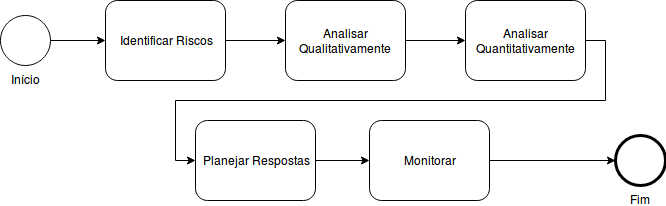
\includegraphics[scale=0.5]{figuras/processo-gerencia-riscos}
	\captionof{figure}{Processo de Gerência de Riscos}
\end{center}

\begin{itemize}
    \item \textbf{Planejar o Gerenciamento dos Riscos}
        \begin{itemize}
            \item \textbf{Objetivo}
            Nesta fase é definido como as atividades de gerenciamento dos riscos serão dirigidas ao longo do projeto \cite{pmbok2004guia}.
            \item \textbf{Ferramentas e técnicas}
            Reuniões e opinião especializada.
        \end{itemize}
    
    \item \textbf{Identificar Riscos}
        \begin{itemize}
            \item \textbf{Objetivo}
            Processo de determinação dos riscos que podem afetar o projeto e de documentação das suas características \cite{pmbok2004guia}.
            \item \textbf{Ferramentas e técnicas}
            What If e análise de premissas.
        \end{itemize}

    \item \textbf{Analisar Qualitativamente}
        \begin{itemize}
            \item \textbf{Objetivo}
            O processo de priorização de riscos para análise ou ação posterior através da avaliação e combinação de sua probabilidade de ocorrência e impacto \cite{pmbok2004guia}.
            \item \textbf{Ferramentas e técnicas}
            Checklist, Avaliação de probabilidade e impacto dos riscos, matriz de probabilidade e impacto.
        \end{itemize}
    \item \textbf{Analisar Quantitativamente}
        \begin{itemize}
            \item \textbf{Objetivo}
            O processo de analisar numericamente o efeito dos riscos identificados nos objetivos gerais do projeto.
            \item \textbf{Ferramentas e técnicas}
            Apresentação de dados e opinião especializada.
        \end{itemize}
    \item \textbf{Planejar Respostas}
        \begin{itemize}
            \item \textbf{Objetivo}
            O processo de desenvolvimento de opções e ações para reduzir as ameaças aos objetivos do projeto.
            \item \textbf{Ferramentas e técnicas}
            Estratégias para riscos negativos ou ameaças e estratégias de respostas de contingência.
        \end{itemize}
    \item \textbf{Monitorar}
        \begin{itemize}
            \item \textbf{Objetivo}
            O processo de implementar planos de respostas aos riscos, acompanhar os riscos identificados, monitorar riscos residuais, identificar novos riscos e avaliar a eficácia do processo de gerenciamento dos riscos durante todo o projeto.
            \item \textbf{Ferramentas e técnicas}
            Reavaliação de riscos, revisão técnica em pares e reuniões.
        \end{itemize}
\end{itemize}


\subsection{Papéis e Responsabilidades}
Os papéis e responsabilidades do projeto foram determinadas de forma que todos os líderes participem em conjunto nas áreas de identificação, no planejamento de respostas e no monitoramento colocando em prática as ferramentas escolhidas.

\subsection{Prazos associados}
Como foi definido no tópico de metodologia, ao iniciar cada sprint será realizada a análise e o planejamento das respostas. O monitoramento será feito ao longo de todo o processo. Mais precisamente, ao início de cada sprint, começará a gerência daquele ciclo de trabalho, acontecerão as análises, planejamentos e reavaliação para mudanças, pedido formal (volátil) e atualização de documentos (volátil).

\subsection{Categoria de Riscos}
No contexto deste projeto, para ter uma visão compacta e de fácil gerenciamento, os riscos foram divididos apenas em internos e externos. Dividir os riscos em categorias facilita a ter uma visão mais ampla dos pontos “fracos” do projeto e que devem possuir uma maior atenção dos gestores.

\subsubsection{Interno}
Fatores internos são atribuições que podem afetar o projeto de dentro do contexto da equipe. São inerentes ao projeto, controlado pelo líder, que utiliza ações e atividades diretas para mitiga-los.[6]

\subsubsection{Externo}
Fatores externos são atribuições que podem afetar o projeto de fora do contexto da equipe. Podem ser influenciados pelo líder, mas não é possível controlá-los [6]. Sendo assim, são colocadas formas de preveção contra esses tipos de riscos.

\subsection{Análise dos Riscos}
Em um Projeto de Engenharia, os riscos podem causar grande impacto caso não sejam bem mapeados e, visto isso, qualquer tipo de risco deve ser identificado e analisado cautelosamente. Devido essa necessidade, foi definido quatro atributos para analisar os riscos (Probabilidade, Impacto, Peso e Prioridade).

Relacionado às possibilidades e chances de acontecimento de determinado risco, foram classificados 5 níveis: Raro, Improvável, Moderado, Provável e Quase Certo. 

Em relação à impacto e quantificando o efeito potencial sobre o risco no projeto, comumente relacionados a escopo, custo, qualidade e tempo foram definidos outros 5 níveis distintos: Insignificante, Baixo, Moderado, Alto e Catastrófico.

Logo após todas as definições, é realizada as de prioridades, onde foram classificados três níveis distintos: Prevenir, Controlar e Mitigar.


\subsection{Definições de Probabilidades e Impactos de Riscos}
Foram definidos faixas de valores e definições. Logo abaixo, foram construídas tabelas para fornecer base ao registro dos riscos.

A equipe deve se reunir para, com base nas experiências, no material de referência e nas ferramentas propostas, definir qual a probabilidade de determinado risco acontecer e seu impacto no projeto. As escalas de probabilidade são definidas em Raro, Improvável, Moderado, Provável e Quase Certo, e as escalas de impacto são definidas em Insignificante, Baixo, Moderado, Alto e Catastrófico.

\begin{table}[htp]
    \centering
    \caption{Pesos para faixas de Probabilidades}
    \label{my-label}
    \begin{tabular}{|l|l|}
    \hline
    \textbf{Probabilidade (P)} & \textbf{Peso} \\ \hline
    Raro(\textless 10\%) & 0.2 \\ \hline
    Improvável (10\% - 25\%) & 0.4 \\ \hline
    Moderado (25\% - 50\%) & 0.6 \\ \hline
    Provável (50\% - 75\%) & 0.8 \\ \hline
    Quase Certo (\textgreater 75\%) & 1.0 \\ \hline
    \end{tabular}
\end{table}

\begin{table}[htp]
    \centering
    \caption{Pesos para faixas de Impacto}
    \label{my-label}
    \begin{tabular}{|p{0.15\linewidth}|p{0.55\linewidth}|p{0.15\linewidth}|}
    \hline
    \textbf{Impacto (I)} & \textbf{Descrição} & \textbf{Peso} \\ \hline
    Insignificante & Quase que imperceptível & 0.05 \\ \hline
    Baixo & Pouca influência no desenvolvimento do projeto & 0.10 \\ \hline
    Moderado & Notável ao projeto, mas sem grandes consequências & 0.20 \\ \hline
    Alto & Dificulta o desenvolvimento do projeto & 0.40 \\ \hline
    Catastrófico & Impossibilita o prosseguimento do projeto & 0.80 \\ \hline
    \end{tabular}
\end{table}

A equipe definiu, usando como base no guia PmBok, que os principais objetivos do projeto são Custo, Tempo, Escopo e Qualidade. Com isso, foi construída uma tabela, com base nas escalas de impacto dos riscos, em que é inserido descrições de condições e tolerâncias dentro de cada objetivo de projeto para que assim, se tenha noção do que pode ocorrer caso o risco não seja controlado.

\begin{table}[htp]
    \centering
    \caption{Condições e Tolerâncias para as Escalas de Impacto de um Risco}
    \label{my-label}
    \begin{tabular}{|p{0.18\linewidth}|p{0.18\linewidth}|p{0.18\linewidth}|p{0.18\linewidth}|p{0.18\linewidth}|}
    \hline
    \textbf{Impacto / Objetivo} & \textbf{Custo} & \textbf{Tempo} & \textbf{Escopo} & \textbf{Qualidade} \\ \hline
    \textbf{Insignificante} & Aumento insignificante & Aumento dentro do esperado & Diminuição insignificante & Degradação insignificante \\ \hline
    \textbf{Baixo} & Aumento dentro do esperado & Aumento negociável & Áreas secundárias afetadas & Somente aplicações muito exigentes são afetadas \\ \hline
    \textbf{Moderado} & Aumento negociável & Trabalho lento & Áreas principais afetadas & Redução requer aprovação,do orientador \\ \hline
    \textbf{Alto} & Recurso com falhas ou defeitos & Produto final incompleto & Redução do escopo,inaceitável para os orientadores & Redução de qualidade inaceitável para os orientadores \\ \hline
    \textbf{Catastrófico} & Recursos inúteis & Produto final é efetivamente inútil & Produto final é efetivamente inútil & Produto final é efetivamente inútil \\ \hline
    \end{tabular}
\end{table}

\subsection{Matriz de Probabilidade e Impacto}
A tabela abaixo, definida como matriz, e baseada nas tabelas 8 e 9, possibilita a definição de um valor de peso para o risco.

\begin{table}[htp]
    \centering
    \caption{Pesos dos Riscos (PxI)}
    \label{my-label}
    \begin{tabular}{|p{0.18\linewidth}|p{0.18\linewidth}|p{0.10\linewidth}|p{0.15\linewidth}|p{0.10\linewidth}|p{0.15\linewidth}|}
    \hline
    \textbf{Impacto / Objetivo} & \textbf{Insignificante} & \textbf{Baixo} & \textbf{Moderado} & \textbf{Alto} & \textbf{Catastrófico} \\ \hline
    \textbf{Raro} & 0.01 & 0.02 & 0.04 & 0.08 & 0.16 \\ \hline
    \textbf{Improvável} & 0.02 & 0.04 & 0.08 & 0.16 & 0.32 \\ \hline
    \textbf{Moderado} & 0.03 & 0.06 & 0.12 & 0.24 & 0.48 \\ \hline
    \textbf{Provável} & 0.04 & 0.08 & 0.16 & 0.32 & 0.64 \\ \hline
    \textbf{Quase Certo} & 0.05 & 0.10 & 0.20 & 0.40 & 0.80 \\ \hline
    \end{tabular}
\end{table}

Com base na matriz elaborada, é possível definir o cenário do projeto para cada peso (PxI).

\begin{table}[htp]
    \centering
    \caption{Faixas de cenários}
    \label{my-label}
    \begin{tabular}{|p{0.18\linewidth}|p{0.17\linewidth}|p{0.15\linewidth}|p{0.15\linewidth}|p{0.15\linewidth}|p{0.15\linewidth}|}
    \hline
    \textbf{Impacto / Objetivo} & \textbf{Insignificante} & \textbf{Baixo} & \textbf{Moderado} & \textbf{Alto} & \textbf{Catastrófico} \\ \hline
    \textbf{Raro} & Equilibrado & Equilibrado & Equilibrado & Alerta & Alerta \\ \hline
    \textbf{Improvável} & Equilibrado & Equilibrado & Alerta & Alerta & Crítico \\ \hline
    \textbf{Moderado} & Equilibrado & Alerta & Alerta & Crítico & Crítico \\ \hline
    \textbf{Provável} & Equilibrado & Alerta & Alerta & Crítico & Crítico \\ \hline
    \textbf{Quase Certo} & Alerta & Alerta & Crítico & Crítico & Crítico \\ \hline
    \end{tabular}
\end{table}

Resposta:
\begin{itemize}
    \item Equilibrado -> Prevenir
    \item Alerta -> Controlar
    \item Crítico -> Mitigar
\end{itemize}

Caso se tenha que escolher entre dois riscos que tenha o mesmo cenário e a mesma resposta, a prioridade é do com o maior valor de peso, e se esse valor também for igual, os riscos analisados devem ser avaliados ao mesmo tempo.

\subsection{Controle e Rastreabilidade}
Utilizando este documento como base, é possível elaborar o Registro dos Riscos (RR) para se ter noção de todos os riscos que podem afetar o projeto de forma negativa ou positiva. Os riscos sendo mapeados no RR, é possível ter a noção da prioridade e forma de controle de cada um criando assim, a rastreabilidade de todos. Para garantir a qualidade das atividades de controle sobre os riscos, serão feitas inspeções informais ao início de cada sprint elaborando assim, um relatório de controle com situação de combate, prioridade e pedidos de mudanças sobre os riscos monitorados.

\chapter{Registro dos Riscos}

\subsection{WhatIf}
\begin{table}[htp]
    \centering
    \caption{WhatIf}
    \label{my-label}
    \begin{tabular}{|p{0.18\linewidth}|p{0.18\linewidth}|p{0.18\linewidth}|p{0.20\linewidth}|p{0.18\linewidth}|}
    \hline
    \textbf{Atividade} & \textbf{O que aconteceria se ?} & \textbf{Causas} & \textbf{Consequências} & \textbf{Observações} \\ \hline
    Construção da estrutura & Quebrasse uma ferramenta & Descuido & Deve-se comprar outra & Quem quebrou paga \\ \hline
    Construção do app & Não for possível integrar com a máquina & Falta de conhecimento & Requisito de bonificação incompleto & Estudo frequente \\ \hline
    Compra de material & Viesse errado ou com defeito & Descuido de quem comprou, erro de fábrica ou descuido da empresa de transporte & Atraso no desenvolvimento e aumento nos custos & Fez a decisão de compra errada sozinho, paga sozinho. Veio com defeito, o grupo paga \\ \hline
    Integração do projeto & Algum subsistema não estiver pronto & Irresponsabilidade dos responsáveis ou falta de conhecimento & Diminuição na nota de todo o grupo & Se estiver dependendo de um subsistema, tente ajudar os responsáveis ao,máximoSe o responsável não estiver trabalhando, avise a equipe para que,todos,avisem os professores \\ \hline
    Desenvolvimento do projeto & Um integrante saisse & Motivos pessoais & Trabalho sem alocação & Todos devem infomar certas ações com bastante antecedência \\ \hline
    Desenvolvimento do projeto & Não tiver o material no galpão & Outro grupo tomou posse ou não tem & Aumento no custo & Procurar se há a disponibilidade do material ou da ferramenta de forma gratuita em algum lugar de Brasília \\ \hline
    \end{tabular}
\end{table}

\subsection{Tabela de Registros}
\begin{table}[!htp]
    \centering
    \caption{Registros dos Riscos}
    \label{my-label}
    \begin{tabular}{|p{0.10\linewidth}|p{0.25\linewidth}|p{0.25\linewidth}|p{0.25\linewidth}|}
    \hline
    \textbf{ID} & \textbf{Descrição} & \textbf{Causa} & \textbf{Impacto descrito} \\ \hline
    R01 & Queima de equipamento por descarga elétrica & Descuido de quem estiver ligando o equipamento & Aumento no custo e tempo do projeto \\ \hline
    R02 & Atraso na entrega de material & Fornecedor não tem ou falha no processo de entrega & Parte do projeto não pode ser feito \\ \hline
    R03 & Erro de dimensionamento dos subsistemas & Descuido do responsável pela atividade & Retrabalho \\ \hline
    R04 & Falha de integração entre o app e a máquina & Falta de conhecimento dos envolvidos & Requisito de bonificação não finalizado \\ \hline
    R05 & Falha de integração dos subsistemas da máquina & Falta de tempo ou conhecimento dos envolvidos & Não haverá um produto para apresentar \\ \hline
    R06 & Material com defeito & Defeito de fábrica ou descuido & Parte do projeto não pode ser feito \\ \hline
    R07 & Integrante se ausenta da disciplina & Causa pessoal & Maior volume de trabalho para os outros membros \\ \hline
    R08 & Não entrega de atividades no prazo & Planejamento falho & Atraso no andamento do projeto \\ \hline
    R09 & Escopo muito grande para o prazo ou orçamento & Pedido ou inexperiência dos integrantes & Estouro de custo e não entrega completa do projeto \\ \hline
    R10 & Inadimplência de algum integrante & Falta de dinheiro & Maior gastos a outros membros \\ \hline
    R11 & Escolha inadequada de componentes /equipamentos & Descuido do responsável pela atividade & Atraso e aumento no custo \\ \hline
    R12 & Mal dimensionamento do consumo elétrico & Descuido do responsável pela atividade & Retrabalho \\ \hline
    R13 & Extravio ou danificação de materiais no galpão & Descuido do responsável pela atividade & Aumento no custo e tempo do projeto \\ \hline
    R14 & Indisponibilidade de equipamentos no galpão & Outro grupo já tomou posse ou esta estragado & Aumento no custo \\ \hline
    R15 & Falta de internet no dia da apresentação & Falha da internet do campus & Ter celulares preparados para rotear \\ \hline
    \end{tabular}
\end{table}

\newpage
\subsection{Análise e Respostas aos Riscos}
\begin{table}[!htp]
    \centering
    \caption{Análise dos Riscos}
    \label{my-label}
    \begin{tabular}{|p{0.10\linewidth}|p{0.18\linewidth}|p{0.15\linewidth}|p{0.10\linewidth}|p{0.15\linewidth}|p{0.18\linewidth}|}
    \hline
    \textbf{ID} & \textbf{Probabilidade} & \textbf{Impacto em nível} & \textbf{P x I} & \textbf{Prioridade} & \textbf{Ação} \\ \hline
    R01 & Queima de equipamento por descarga elétrica & Baixo & 0.06 & Alerta & Controlar - Manter a atenção ao ligar todos os equipamentos \\ \hline
    R02 & Atraso na entrega de material & Alto & 0.32 & Crítico & Mitigar - Procurar todos os componentes dentro de brasília e os que não houverem, pedir bem antes e deixar mais um fornecedor a pronta entrega \\ \hline
    R03 & Erro de dimensionamento dos subsistemas & Alto & 0.32 & Crítico & Mitigar - Procura de professores e apresentação prévia dos dimensionamentos realizados a todo o time de estrutura \\ \hline
    R04 & Falha de integração entre o app e a máquina & Alto & 0.24 & Crítico & Mitigar - Plano de estudo prévio e boa relação entre os integrantes de software e eletrônica \\ \hline
    R05 & Falha de integração dos subsistemas da máquina & Catastrófico & 0.80 & Crítico & Mitigar - Manter trabalho de subsistemas atualizados entre si e iniciar a integração logo que puder \\ \hline
    R06 & Material com defeito & Baixo & 0.06 & Alerta & Controlar - Evitar comprar material de fora de brasília para ter a possibilidade de teste na hora da compra e deixar mais um fornecedor a pronta entrega \\ \hline
    R07 & Integrante se ausenta da disciplina & Moderado & 0.08 & Alerta & Controlar - Manter constante comunicação entre os integrantes \\ \hline
    R08 & Não entrega de atividades no prazo & Catastrófico & 0.32 & Crítico & Mitigar - Seguir planejamento e rigorisidade em datas \\ \hline
    R09 & Escopo muito grande para o prazo ou orçamento & Alto & 0.32 & Crítico & Mitigar - Avaliar sempre alternativas de equipamentos e componentes mais baratos e dialogar formalmente e bem com os professores \\ \hline
    R10 & Inadimplência de algum integrante & Moderado & 0.12 & Alerta & Controlar - Conversar previamente com todos sobre situação financeira e anotações plenas de todos as entradas e saídas do caixa de forma a deixar explícito a contribuição para os professores \\ \hline
    R11 & Escolha inadequada de componentes /equipamentos & Alto & 0.16 & Alerta & Controlar - Reunião de avaliação sobre cada componente \\ \hline
    R12 & Mal dimensionamento do consumo elétrico & Alto & 0.24 & Crítico & Mitigar - Empenho do responsável e procura de professores \\ \hline
    R13 & Extravio ou danificação de materiais no galpão & Catastrófico & 0.48 & Crítico & Mitigar - Manter histórico de atividades feitas no galpão e fotos da máquina todos os dias de trabalho \\ \hline
    R14 & Indisponibilidade de equipamentos no galpão & Moderado & 0.20 & Crítico & Mitigar - Procurar locais que possam ter o equipamento para,aluguel ou uso gratuito \\ \hline
    R15 & Falta de internet no dia da apresentação & Insignificante & 0.05 & Alerta & Controlar - Membros rotearem no celular \\ \hline
    \end{tabular}
\end{table}

\newpage
\subsection{Checklist}
\begin{table}[!htp]
    \centering
    \caption{Checklist}
    \label{my-label}
    \begin{tabular}{|p{0.15\linewidth}|p{0.15\linewidth}|p{0.25\linewidth}|p{0.15\linewidth}|}
    \hline
    \textbf{Risco} & \textbf{Situação} & \textbf{Resposta} & \textbf{Resultado} \\ \hline
    R03 & Identificando & Mitigar - Procura de professores e apresentação prévia dos dimensionamentos realizados a todo o time de estrutura & Em andamento \\ \hline
    R04 & Identificando & Mitigar - Plano de estudo prévio e boa relação entre os integrantes de software e eletrônica & Em andamento \\ \hline
    R05 & Identificando & Mitigar - Manter trabalho de subsistemas atualizados entre si com reuniões presenciais semanais e iniciar a integração logo que puder & Prevenindo \\ \hline
    R06 & Identificando & Controlar - Evitar comprar material de fora de brasília para ter a possibilidade de teste na hora da compra e deixar mais um fornecedor a pronta entrega & Controlando \\ \hline
    R14 & Identificando & Mitigar - Procurar locais que possam ter o equipamento para,aluguel ou uso gratuito & Em andamento \\ \hline
    R15 & Identificando & Controlar - Membros rotearem no celular & Controlando \\ \hline
    \end{tabular}
\end{table}

\chapter{Documento de Visão}

\subsection{Introdução}
O documento de visão define o escopo de alto nível e o propósito do software a ser desenvolvido. Esse visa estabelecer as expectativas e reduzir os riscos do produto protegendo o cliente e os desenvolvedores do projeto.

\subsubsection{Finalidade}
O documento presente tem, por finalidade, apresentar e estabelecer uma visão ampla sobre o aplicativo da Máquina de Reciclagem de modo que deixe claro sua proposta, características e utilidade.

\subsubsection{Escopo}
O App - Máquina de Reciclagem: aplicativo de gerenciamento de contas de usuários e suas bonificações. É um projeto desenvolvido por alunos (Elmar Roberto, Gabriel de Souza e Henrique Dutra) de Engenharia de Software, Faculdade UnB Gama (FGA) da Universidade de Brasília (UnB).

Esta plataforma vem para auxiliar no uso da Máquina Automática de Reciclagem, suprindo a necessidade de automatização da gerência de dados dos usuários. Os dados gerenciados são as bonificações vindas dos depósitos de garrafas, onde cada garrafa fornece uma quantia específica de crédito para descontos em estabelecimentos. É um trabalho baseado em projetos parecidos onde segue as mesmas propostas gerais, interligar tecnologicamente e financeiramente as pessoas que depositam garrafas com a máquina e seus dados gerados.

A máquina será usada para armazenar as garrafas recicláveis, sendo esta estabelecida em qualquer estabelecimento que tenha suporte para integração com o app. A descrição detalhada da máquina esta nos tópicos das outras engenharias.

O app, de forma geral, funcionará da seguinte maneira: iniciada a utilização da máquina, a mesma deverá ler um QR Code gerado pelo App, onde este servirá como reconhecimento do usuário ali presente. Após tal reconhecimento, o usuário deverá inserir as garrafas e o sistema da máquina deverá validar e contabilizar cada uma. Terminada a inserção, o app deverá ser atualizado automaticamente com os frutos das ações descritas e fornecer ao usuário os créditos que servirão futuramente para descontos nos produtos do estabelecimento em que a máquina está instalada.

\subsubsection{Definições, Acrônimos e Abreviações}

\begin{itemize}
    \item UnB - Universidade de Brasília
    \item FGA - Faculdade UnB Gama
\end{itemize}

\subsubsection{Visão Geral do documento}
Neste documento de visão estão descritos os detalhes do planejamento e construção do software proposto. O documento apresentará os motivos que levaram o desenvolvimento do aplicativo que dará apoio ao projeto da Máquina de Reciclagem, apresentando a problemática, bem como quem está envolvido, desenvolvedores e usuários, e as funções do produto.

\subsection{Posicionamento}

\subsubsection{Oportunidade de Negócio}
Pelo mundo já foram criadas algumas máquinas com a finalidade de auxílio na reciclagem, mas as formas de ganho ao usuário são diversificadas, algumas dão a oportunidade apenas de compartilhamento de seus feitos em redes sociais, outras trocam as garrafas pets por rações para animais de estimação, tem as que dão dinheiro e algumas fornecem descontos em estabelecimentos, sendo este projeto do último tipo citado.

Sendo assim, o aplicativo oferecerá um serviço de facilitador no controle de bonificações ao usuário onde tal bonificação poderá ser um tipo de atrativo e marketing ao estabelecimento.

\subsubsection{Descrição do Problema}

\begin{table}[htp]
    \centering
    \caption{Descrição do Problema}
    \label{my-label}
    \begin{tabular}{|p{0.25\linewidth}|p{0.65\linewidth}|}
        \hline
        O problema de     & Grande dispêndio de tempo para organizar tais dados de crédito de forma manual ou em um sistema único do estalecimento em que o usuário teria que se locomover até o local para verificar seus dados. \\ \hline
        Afeta             & A agilidade de controle dos créditos e interesse do usuário no uso da máquina \\ \hline
        Cujo impacto é    & O alto custo de tempo no controle e perda de usuários por falta de comodidade. \\ \hline
        Uma solução seria & A otimização e automoção do controle de tais créditos \\ \hline
    \end{tabular}
\end{table}

\subsubsection{Sentença de Posição do Produto}

\begin{table}[htp]
    \centering
    \caption{Sentença de Posição do Produto}
    \label{my-label}
    \begin{tabular}{|p{0.25\linewidth}|p{0.65\linewidth}|}
        \hline
        Para              & Clientes do estabelecimento. \\ \hline
        Que               & Desejam receber créditos pelas ações de reciclagem  \\ \hline
        O App - Máquina de Reciclagem    & É um aplicativo Android e IOS \\ \hline
        Que & Visa automatizar o controle de créditos do usuário  \\ \hline
        Diferente de & Recicletool \cite{recicletool} e Pugedon \cite{pugedon}  \\ \hline
        Parecido com & Retorna Machine \cite{retornaMachine} \\ \hline
        Nosso produto & Tem como objetivos atrair as pessoas à ação de reciclagem e fornecer controle automático aos seus dados de créditos de descontos em produtos. \\ \hline
    \end{tabular}
\end{table}

\subsection{Descrições dos Envolvidos e dos Usuários}
Os principais envolvidos neste projeto serão por parte da equipe de desenvolvimento, programadores e gestores e os orientadores da disciplina onde o produto está sendo construído.

Já os usuários que irão interagir comercialmente, serão os clientes dos estabelecimentos e os próprios estabelecimentos.

\subsubsection{Resumo dos Envolvidos}

\begin{table}[htp]
    \centering
    \caption{Resumo dos Envolvidos}
    \label{my-label}
    \begin{tabular}{|p{0.25\linewidth}|p{0.35\linewidth}|p{0.35\linewidth}|}
        \hline
        \multicolumn{1}{|c|}{\textbf{Nome}} & \multicolumn{1}{c|}{\textbf{Descrição}} & \multicolumn{1}{c|}{\textbf{Responsabilidade}} \\ \hline
        Equipe de  Desenvolvimento          &        Estudantes da disciplina Projeto Integrador II, ministrada na Universidade do Gama (FGA - UnB).                                 &               Desenvolvimento e testes do Software.                                 \\ \hline
        Equipe de Gestão de Projetos                                    &     Estudantes da disciplina Projeto Integrador II, ministrada na Universidade do Gama (FGA - UnB).                                    &           Gerenciamento do desenvolvimento do software, identificando problemas e indicando possíveis soluções.                                     \\ \hline
        Cliente                                   &             Professores da disciplina.                            &         Esclarecer as aplicações do software.                                       \\ \hline
        Patrocinador                                    &         Professores da Universidade de Brasília, no campus Faculdade Gama (FGA - UnB), da disciplinas Projeto Integrador II.                                &       Orientar as equipe de desenvolvimento e gestão em eventuais dúvidas.                                         \\ \hline
    \end{tabular}
\end{table}

\subsubsection{Resumo dos Usuários}

\begin{table}[htp]
    \centering
    \caption{Resumo dos Usuários}
    \label{my-label}
    \begin{tabular}{|p{0.25\linewidth}|p{0.35\linewidth}|p{0.35\linewidth}|}
        \hline
        \multicolumn{1}{|c|}{\textbf{Nome}} & \multicolumn{1}{c|}{\textbf{Descrição}} & \multicolumn{1}{c|}{\textbf{Responsabilidade}} \\ \hline
        Clientes do estabelecimento & Clientes que buscam descontos no estalecimento. & Ter acesso a conta individual e visualização e controle de créditos já adquiridos. \\ \hline
    \end{tabular}
\end{table}

\subsubsection{Principais Necessidades dos Usuários e dos Envolvidos}

Os usuários utilizarão a aplicação em seu celular com o sistema operacional Android ou IOS.

\subsubsection{Perfis dos Envolvidos}

\subsubsubsection{Equipe de Gestão}

\begin{table}[htp]
    \centering
    \caption{Equipe de Gestão}
    \label{my-label}
    \begin{tabular}{|p{0.40\linewidth}|p{0.60\linewidth}|}
        \hline
        Representantes    & Elmar Roberto Caixeta Filho, Gabriel de Souza Clímaco e Henrique Dutra. \\ \hline
        Descriçao    & Gerenciamento de projeto. \\ \hline
        Tipo    & Estudantes da matéria Projeto Integrador II ministrada na Universidade do Gama (FGA - UnB). \\ \hline
        Responsabilidades    & Monitorar o desenvolvimento. Definir prazos para as atividades propostas. \\ \hline
        Critérios de Sucesso    & Manter os prazos estabelecidos sem atraso, e gerenciar a qualidade do software em desenvolvimento, finalizando o projeto no tempo estipulado. \\ \hline
        Envolvimento    & Alto. \\ \hline
        Problemas/Comentários    & Organizar prazos e metas de acordo com o tempo disponível. \\ \hline
    \end{tabular}
\end{table}

\subsubsubsection{Equipe de Desenvolvimento}

\begin{table}[htp]
    \centering
    \caption{Equipe de Desenvolvimento}
    \label{my-label}
    \begin{tabular}{|p{0.40\linewidth}|p{0.60\linewidth}|}
        \hline
        Representantes    & Elmar Roberto Caixeta Filho, Gabriel de Souza Clímaco e Henrique Dutra. \\ \hline
        Descriçao    & Desenvolvimento do Software. \\ \hline
        Tipo    & Estudantes da matéria Projeto Integrador II ministrada na Universidade do Gama (FGA - UnB). \\ \hline
        Responsabilidades    & Desenvolver, testar e implantar o software. \\ \hline
        Critérios de Sucesso    & Finalizar o desenvolvimento e realizar a entrega do aplicativo no tempo estipulado. \\ \hline
        Envolvimento    & Alto. \\ \hline
        Problemas/Comentários    & Alta experiência dos desenvolvedores. \\ \hline
    \end{tabular}
\end{table}

\subsubsubsection{Cliente}

\begin{table}[htp]
    \centering
    \caption{Cliente}
    \label{my-label}
    \begin{tabular}{|p{0.40\linewidth}|p{0.60\linewidth}|}
        \hline
        Representantes    & Professores da disciplina. \\ \hline
        Descriçao    & Professores da Universidade de Brasília, no campus Faculdade Gama (FGA - UnB). \\ \hline
        Tipo    &  Cliente especialista nos conhecimentos técnicos. \\ \hline
        Responsabilidades    & Validar os principais requisitos.  \\ \hline
        Critérios de Sucesso    & A correta validação de requisitos. \\ \hline
        Envolvimento    & Alto. \\ \hline
        Problemas/Comentários    & . \\ \hline
    \end{tabular}
\end{table}

\subsubsubsection{Orientadores}

\begin{table}[htp]
    \centering
    \caption{Orientadores}
    \label{my-label}
    \begin{tabular}{|p{0.40\linewidth}|p{0.60\linewidth}|}
        \hline
        Representantes    & Professores da disciplina \\ \hline
        Descriçao    & Professores da Universidade de Brasília, no campus Faculdade Gama (FGA - UnB), da disciplina Projeto Integrador II. \\ \hline
        Tipo    & Orientadores e avaliadores que darão suporte a respeito do desenvolvimento do aplicativo. \\ \hline
        Responsabilidades    & Avaliar a equipe e orientar em eventuais dúvidas \\ \hline
        Critérios de Sucesso    & Observar o sucesso da equipe de desenvolvimento. \\ \hline
        Envolvimento    & Médio. \\ \hline
        Problemas/Comentários    & . \\ \hline
    \end{tabular}
\end{table}

\subsubsection{Perfis dos Usuários}

\subsubsubsection{Clientes}

\begin{table}[htp]
    \centering
    \caption{Clientes}
    \label{my-label}
    \begin{tabular}{|p{0.40\linewidth}|p{0.60\linewidth}|}
        \hline
        \multicolumn{1}{|c|}{\textbf{Representantes}} & \multicolumn{1}{c|}{\textbf{Clientes do estabelecimento}} \\ \hline
        Descrição    & Pessoas que desejam usar a máquina e adquirir os créditos. \\ \hline
        Tipo    & Possuidores de contas individuais e recebedores de créditos. \\ \hline
        Responsabilidades    & Receber bonificações e consumir os produtos da empresa. \\ \hline
        Critérios de Sucesso    & Ter total controle e privacidade de seus créditos e usá-los. \\ \hline
        Envolvimento    & Alto. \\ \hline
        Problemas/Comentários    & Não ter conexão com a internet. \\ \hline
    \end{tabular}
\end{table}

\subsubsection{Principais Necessidades dos Usuários ou dos Envolvidos}

\begin{table}[htp]
    \centering
    \caption{Principais Necessidades}
    \label{my-label}
    \begin{tabular}{|p{0.20\linewidth}|p{0.20\linewidth}|p{0.20\linewidth}|p{0.20\linewidth}|p{0.20\linewidth}|}
    \hline
    \multicolumn{1}{|c|}{\textbf{Necessidade}} & \multicolumn{1}{c|}{\textbf{Prioridade}} & \multicolumn{1}{c|}{\textbf{Preocupação}} & \multicolumn{1}{c|}{\textbf{Solução Proposta}} & \multicolumn{1}{c|}{\textbf{Solução Atual}} \\ \hline
    Automatizar o controle de crédito          & Alta                                     & -                                         & -                                              & -                                           \\ \hline
    \end{tabular}
\end{table}

\subsubsection{Alternativas e Concorrências}

\subsubsubsection{Recicletool}
Máquina desenvolvida para captação de resíduos sólidos, a ferramenta busca ajudar não apenas na reutilização dos materiais recicláveis, mas também às pessoas que vivem disto, como catadores e cooperativas, gerando renda para o usuário. Basta que o usuário se cadastre, através do número do seu celular, na própria máquina. Em seguida, ele deve depositar os resíduos sólidos, como garrafas PET ou latinhas de refrigerante. A máquina automaticamente vai somando o valor gerado pelo usuário

\subsubsubsection{Pugedon}
Máquina automática que estimula a reciclagem e ao mesmo tempo ajuda a alimentar os cães e gatos de Istambul. Para cada garrafa ou lata inserida no equipamento, a máquina libera uma porção de ração.

\subsubsubsection{Retorna Machine}
Máquina de reciclagem que gera desconto no supermercado. Quem deposita as embalagens vazias ganha incentivos como desconto na conta de luz e créditos no sistema de transporte público da cidade, dentre outros serviços. Além disso, se a embalagem for de desodorante, a recompensa é um cupom de 30\% de desconto para a compra de novos produtos de marcas específicas.

\subsection{Descrição da Solução}

\subsubsection{Perspectiva do Produto}
O aplicativo tem como objetivo incentivar a reciclagem por meio de bonificações de descontos em produtos consumíveis.

\subsubsection{Resumo dos Recursos}
\begin{table}[htp]
    \centering
    \caption{Resumo dos Recursos}
    \label{my-label}
    \begin{tabular}{|p{0.40\linewidth}|p{0.60\linewidth}|}
        \hline
        \multicolumn{1}{|c|}{\textbf{Benefício para o Cliente}} & \multicolumn{1}{c|}{\textbf{Recursos de suporte}} \\ \hline
        Gerenciamento automático de créditos    & O aplicativo, através das respostas de inserção de garrafas da máquina, mantém os créditos indiduais de cada cliente. \\ \hline
        Monitora a constribuição dos usuários    & Mantém visível o quanto um cliente está ajudando na reciclagem. \\ \hline
    \end{tabular}
\end{table}

\subsection{Recursos do Produto}
A aplicação do App - Máquina de Reciclagem oferece as seguintes funcionalidades:

\begin{itemize}
    \item Manter Perfil de Usuário.
    \item Gerênciar créditos dos usuários;
    \item Viabilizar visualização de histórico de depósitos;
\end{itemize}

\subsection{Requisitos Funcionais}

\begin{table}[htp]
    \centering
    \caption{Requisitos Funcionais}
    \label{my-label}
    \begin{tabular}{|p{0.25\linewidth}|p{0.35\linewidth}|p{0.35\linewidth}|}
        \hline
        \multicolumn{1}{|c|}{\textbf{ID}} & \multicolumn{1}{c|}{\textbf{Descrição}} & \multicolumn{1}{c|}{\textbf{Prioridade}} \\ \hline
        RF01 & Visualizar Pontuação & Alta \\ \hline
        RF02 & Visualizar Garrafa validada & Média \\ \hline
        RF03 & Visualizar histórico de operações & Média \\ \hline
        RF04 & Editar perfil & Alta \\ \hline
    \end{tabular}
\end{table}

\subsection{Restrições}

\begin{itemize}
    \item Uso da Internet.
\end{itemize}

\subsection{Intervalos de Qualidade}

\subsubsection{Requisitos de Implementação}
Para a implementação do projeto em plataforma Android e IOS com a linguagem JavaScript e o Framework VueJS, será utilizado o modelo arquitetural de Componentes com base no MVVM, empregando o modelo de desenvolvimento baseado em componentes com o amparo do Framework Quasar. O Rethink será o Banco de Dados.

\subsubsection{Requisitos de Sistema}
Esta aplicação deverá ser acessada através de um dispositivo mobile em que o sistema operacional é o Android ou IOS.

\subsubsection{Requisitos de Design}
A composição deste software será feita de maneira a tornar sua utilização autoexplicativa e fácil, para acesso em tempo real, ou seja, atendendo todas as especificações de boas práticas referentes à experiência de usuário.

\subsubsection{Requisitos de Portabilidade}
O sistema será, exclusivamente, para celulares com a plataforma Android e IOS ou superiores, sendo disponibilizado na loja online Google Play.

\subsubsection{Requisitos de Confiança}
A aplicação obriga-se a mostrar as informações relativas ao perfil acessado.

\subsubsection{Requisitos de Privacidade}
Não haverá exposição pública de qualquer dado pessoal, exclusivo o nome do usuário.

Todos os dados referentes as garrafas, descontos e usuários serão arquivados no banco de dados do grupo de desenvolvedores, onde será de inteira responsabilidade destes e da empresa a não divulgação.

\chapter{Documento de Arquitetura}
\subsection{Introdução}
Passada a elicitação de requisitos, é necessário a especificação da arquitetura do software a ser desenvolvido, implicando em uma otimização do entendimento por parte dos desenvolvedores sobre os requisitos e principalmente sobre a estrutura.

\subsection{Escopo}
O software a ser projetado tem como conceito a automatização da gerência de bonificações das pessoas que utilizam a máquina automática de reciclagem. A arquitetura escolhida deve ser baseada na ideia da relação de um cliente, sua interface de uso, uma camada da gerência das requisições de dados, no caso, pode ser uma API/Servidor e o Banco de Dados.

\subsection{Visão Geral}
O documento segue a seguinte estrutura:

\begin{itemize}
    \item Introdução
    \item Representação Arquitetural
    \item Metas e Restrições da Arquitetura
    \item Visão de Casos de Uso
    \item Visão Lógica
    \item Visão de Implementação
\end{itemize}

\subsection{Definições e Acrônimos}
\begin{itemize}
    \item \textbf{UC:} Introdução
    \item \textbf{MVVM:} Representação Arquitetural
\end{itemize}

\subsection{Representação Arquitetural}

\subsubsection{Visão Geral}
De forma geral, o padrão de arquitetura é a Arquitetura em N Camadas baseada na Arquitetura Cliente Servidor, mais precisamente, no caso serão 3 camadas, camada de apresentação, aplicação(API) e dados. Por cima deste padrão será aplicado o estilo arquitetural REST. Esse conjunto de padrão abrangem de forma completa os requisitos macros de estrutura do projeto.

As tecnologias escolhidas para rodarem em cima deste modelo, foram o Vue JS que fornece suporte para o uso das linguagens padronizadas para desenvolvimento front-end, são
elas, JavaScript, HTML5 e CSS3, o Quasar que é um framework Vue de desenvolvimento front-end e fornece recursos para desenvolvimentos de aplicações web e mobile(IOS e Android), o Node JS para fazer o papel de servidor das regras de negócio e o Banco de Dados RethinkDB, banco não relacional que fará o papel de servidor de dados.

É interessante colocar em pauta que as tecnologias de front-end já citadas se encaixam bem nas restrições e requisitos não-funcionais do projeto, além de terem sido escolhidas pela experiência do time. Suas justificativas técnicas estão elucidadas nos próximos tópicos.

Em relação a visão de caso de uso e lógica, o Vue possui um padrão de desenvolvimento chamado Model View ViewModel (MVVM) que tem uma ideia arquitetural geral parecida com o N Camadas que é de separar a parte Visão do projeto das Regras de Negócio, onde essa estrutura tem uma descrição bem interessante sobre a visão de processo arquitetural do projeto.

Já na visão de implantação, a comunicação com o hardware do projeto será possível utilizando da camada central da arquitetura, a API, sendo este ponto explicado em tópicos posteriores, mas de modo geral a camada central e a camada de dados serão responsáveis pela comunicação completa do software e do hardware.

\subsubsection{Descrição e Representação Técnica}
Segundo o arquiteto Christopher Alexanderv \cite{livroPadroesArq}, cada padrão é formado por três regras, a sua relação com o contexto, com o problema e com a solução, sendo assim, é interessante descrever esses três tópicos para o melhor entendimento da escolha arquitetural. O software a ser desenvolvido possui restrições e características que podem ser problemáticas em seu desenvolvimento, o sistema possui interação constante de assuntos de baixo nível com os de alto nível, onde a parte de baixo de nível estará em constante comunicação com o hardware e parte de alto nível estará sempre em contato com o usuário. Como haverá essa alta interação entre os níveis, haverá fluxo constante de pedidos entre os níveis e do hardware. O suporte para comunicação deverá ser aberto para diversos e diferentes periféricos, como exemplo a rapsberry PI, isto também se torna um problema em pontos de reutilização, coesão e pouco acoplamento.

Então, segundo o livro de Wiley\cite{livroPadroesArq} e estudo postado pela UFCG\cite{nCamadas}, estes são problemas que vieram a ser solucionados com o uso do padrão arquitetural em Camadas, onde a solução para estes problemas está em dividir o sistema justamente em camadas e partições, onde uma camada é subsistema que agrega valor ao sistema e partições são subsistemas paralelos a outros subsistemas \cite{nCamadas}. Para solucionar o problema de comunicação a diferentes periféricos, foi-se adotado o padrão Cliente Servidor usando o estilo arquitetural REST, onde este padrão pode ser descrito como uma estrutura em Camadas abrangendo a diferentes protocolos e formas de comunicação sem perder a coesão e reutilização por conta das requisições HTTP universais.

A quantidade de camadas é definida baseada na necessidade de serviços a serem disponibilizados, no caso deste projeto, sabe-se que haverá os serviços disponibilizados pelo aplicativo, os serviços disponibilizados referentes à aplicação que de forma geral é a interface de acesso aos dados do sistema e os serviços de dados. A partir disso é evidente que em questão serão 3 camadas como segue a representação abaixo.

\begin{figure}[!ht]
	\centering
		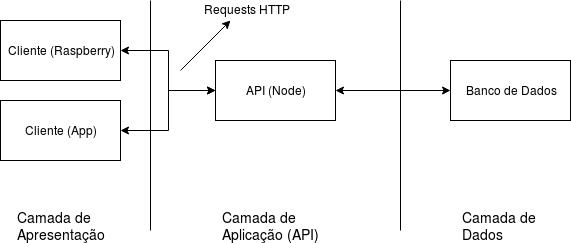
\includegraphics[scale=0.6]{figuras/software/3-estrutura-camadas.png}
	\caption{Estrutura em Camadas}
\end{figure}

\subsection{Visão de Caso de Uso}
\begin{table}[htp]
    \centering
    \caption{Relação da arquitetura com casos de uso}
    \label{my-label}
    \begin{tabular}{|p{0.40\linewidth}|p{0.60\linewidth}|}
        \hline
        \multicolumn{1}{|c|}{\textbf{UC}} & \multicolumn{1}{c|}{\textbf{Descrição na Arquitetura}} \\ \hline
        Visualizar pontuação    & Cliente acessa a camada de apresentação e o sistema faz a requisição dos dados por meio da API. Em caso de incremento de pontos, esse incremento deve ocorrer em tempo real \\ \hline
        Visualizar garrafa validada    & Cliente acessa a camada de apresentação e o sistema faz a requisição dos dados por meio da API esperando a resposta da máquina. Essa resposta é apresentada em tempo real ao usuário \\ \hline
        Visualizar histórico de operações    & Cliente acessa a camada de apresentação e o sistema faz a requisição dos dados por meio da API \\ \hline
        Editar Perfil    & Cliente acessa a camada de apresentação e ele mesmo faz uma requisição de atualização no banco por meio da API \\ \hline
        Gerar QR-Code    & O aplicativo gera o QR-Code por meio do cpf \\ \hline
        Gerenciar Operações    & O sistema gere as operações por meio das requisições REST \\ \hline
        Gerenciar Login    & Atividade envolve requisição de salvamento de usuário por meio de nova inserção ou atualização. O sistema mantém a sessão do usuário. \\ \hline
    \end{tabular}
\end{table}

\subsection{Visão Lógica}
Tendo em vista sua flexibilidade, comunidade bem estabelecida (o que permite maior suporte ao desenvolver) e reatividade, foi escolhido o framework Vue.js para o desenvolvimento da aplicação que será utilizada pelo usuário. Como esta aplicação deve também contemplar o escopo de um aplicativo mobile, optou-se por utilizar o Quasar, o qual é um framework para Vue.js que permite o desenvolvimento de aplicações mobile, além de oferecer uma biblioteca de componentes prontos, que facilitam na hora do desenvolvimento.

Para desenvolvimento da API, escolheu-se o Node.js devido a sua facilidade de desenvolver aplicações em tempo real por meio de websockets. Já para os websockets, optou-se por utilizar o Socket.io, por se tratar de uma das maiores bibliotecas de comunicação em tempo real dentro do ambiente do Node.js. Já para o Banco de Dados, optou-se por utilizar o RethinkDB, pois o mesmo é não relacional, o que facilita sua integração com o Node.js, porém, ele possui algumas das vantagens dos bancos relacionais, como a relação entre duas entidades, algo que será necessário no projeto, vide o diagrama de classes abaixo.

Apesar de não possuir nenhuma tecnologia com o cunho orientado a objetos, elaborou-se um diagrama de classes para elucidar como será a relação entre as entidades do sistema.

\begin{figure}[!ht]
	\centering
		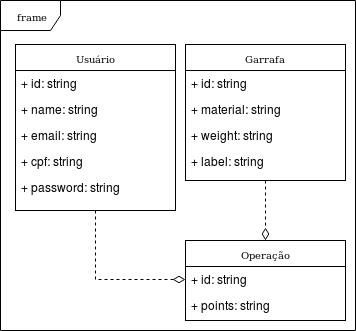
\includegraphics[scale=0.6]{figuras/software/4-diagrama-de-classes.png}
	\caption{Diagrama de Classes}
\end{figure}

As entidade são Usuário, Garrafa e Operação. A entidade Usuário se trata daquele que usará o aplicativo e se identificará por meio de um QR Code. A Garrafa se trata das garrafas que vão ser pré cadastradas no sistema e que serão identificadas também através de um QR Code. A Operação consta na inserção de garrafas na máquina, a qual será a fonte dos pontos do usuário. A Operação por sua vez apresenta uma relação de composição com Usuário e com Garrafa, de modo que ela não existe sem as duas entidades, mas as duas entidades não são dependentes de sua existência. Vale ressaltar que uma Operação pode ser compostas de várias garrafas, porém estará atrelada a um único usuário.

\subsection{Visão de implementação}

\subsubsection{App}
Por se tratar de um projeto baseado no framework Vue.js, a arquitetura do sistema será construída com base na arquitetura proposta pelo framework. Apesar de não ser estritamente baseado no MVVM (detalhada no subsistema de software na seção de planejamento), a arquitetura do Vue foi desenhada de acordo com esse modelo arquitetural. Dito isso, esse modelo funcionará da seguinte forma:

\subsubsection{View}
A camada da view possui uma arquitetura baseada em componentes, onde um componente pode ser definido como uma instância reusável do Vue, uma fração de uma interface completa. Tudo que o usuário vê é, necessariamente, um componente. Os componentes são independentes entre si, apesar de coexistirem, cada um no seu próprio espaço, com seus próprios métodos, suas próprias chamadas de API, sua própria estrutura. A independência dos componentes permite também sua reusabilidade, implementando assim o princípio DRY (don't repeat yourself) de desenvolvimento, o que facilita futuras manutenções.

Diferentemente da arquitetura MVC (Model-View-Component) que separa as camadas da aplicação de maneira horizontal, a arquitetura baseada em componentes separa o as camadas do sistema (no caso desse projeto, da View) de maneira vertical. Em outras palavras, enquanto no MVC existe uma camada responsável apenas por mostrar os dados e outra que recupera os dados a serem mostrados, na arquitetura baseada em componentes tudo isso acontece no mesmo nível arquitetural (geralmente a View), e, como já mencionado, as informações respectivas a um componente estão definidas na instância daquele componente. 

Para melhor elucidação da arquitetura descrita, considere o seguinte exemplo de uma aplicação cujo o escopo é uma lista de afazeres, onde a lista possui itens que podem ser excluídos ou editados e um footer com ações de cunho global e outras informações. A estrutura dessa aplicação na arquitetura baseada e componentes seria a seguinte:

\begin{figure}[!ht]
	\centering
		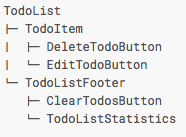
\includegraphics[scale=0.6]{figuras/software/5-arquitetura-todo.png}
	\caption{Arquitetura TODO}
\end{figure}

Onde cada um desses elementos é um componente. O TodoList é o componente onde todos os outros componentes serão adicionados. O TodoItem é um componente que será reusado para cada item da lista de afazeres, de forma que cada TodoItem possuíra um componente DeleteTodoButton e EditTodoButton, que terá a função de excluir e editar um item, respectivamente. Por fim, a TodoList possuirá ainda um componente TodoFooter, o qual possuirá os componentes ClearTodosButton, responsável por limpar todos os afazeres e TodoListStatistics, responsável por mostrar estatísticas dos afazeres (quantos já foram concluídos, por exemplo).

Os componentes foram arquitetados é da seguinte forma:

\begin{figure}[!ht]
	\centering
		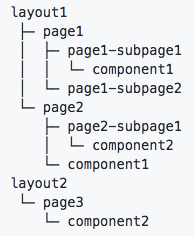
\includegraphics[scale=0.6]{figuras/software/6-arquitetura-componentes-projeto.png}
	\caption{Arquitetura em Componente}
\end{figure}

Haverá um componente layout diferente que irá agrupa um conjunto de páginas. Para cada página, haverá um componente page, que pode ou não conter subcomponentes específicos à sua implementação. Além disso, haverá uma série de componentes que poderão ser reutilizados por vários outros componentes. Esse padrão foi adotado com base na escolha do framework Quasar, tendo em vista que é o padrão sugerido pelo mesmo e que permite melhor
desfrutar de suas utilidades.\cite{arquiteturaCompView} \cite{estruturaQuasar}
 
\subsubsection{Model}
O papel de model é exercido pela store da aplicação. A store nada mais é do que um padrão de gerenciamento de estado para a aplicação de um modo geral, sendo consultado e manipulado pela camada da View. Ele serve como uma centralização de uma biblioteca para todos os componentes em uma aplicação, com regras que garantem que o estado só possa ser mutado de forma previsível. A store, por sua vez, é implementada do Vue através do Vuex.

A arquitetura do Vuex é uma arquitetura baseada em módulos, onde um módulo representa, de um modo geral, uma entidade do sistema.

Segue um diagrama que representa a arquitetura da store:

\begin{figure}[!ht]
	\centering
		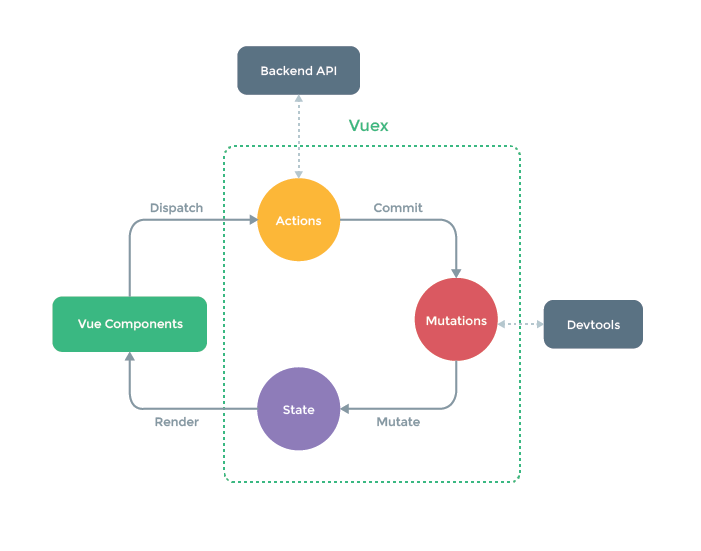
\includegraphics[scale=0.5]{figuras/software/7-vuex.png}
	\caption{Vuex}
\end{figure}

O estado, que consiste em um objeto Javascript, é armazenado no State, o qual é acessado pelo componente através de um Getter, que é uma função cujo único propósito é retornar um valor desejado do estado armazenado no State. O componente, caso deseje consultar uma API externa ou alterar o estado contido no State, deve chamar uma Action, que nada mais é do que um método. A Action por sua vez chamará a API caso necessário e, se for o caso, alterar o estado através de uma Mutation. Da mesma forma que um Getter possui um objetivo único, uma Mutation também segue esse padrão; no entanto, o objetivo da Mutation é apenas alterar um valor específico do State. 

Essa arquitetura se mantém para todo módulo da store. \cite{vuex}

\subsubsection{ViewModel}
A camada da ViewModel funciona como um intermediário entre a camada da View e a camada da Model. No Vue.js, quem faz esse papel de intermediário é a instância global Vue instanciada sempre no começo do projeto. Ao se criar tal instância, é passado um objeto de configuração que determina o seu comportamento.

Como este projeto faz uso do framework Quasar, não há a criação da instância em si, há apenas o objeto de configuração e o framework se encarrega de criar a instância com a composição desejada.\cite{vuejs}

\subsection{API}
A API, por se tratar de um projeto Node.js permite que a arquitetura seja moldada de acordo com a solução e não com base na tecnologia \cite{nodejs}, e por ser uma aplicação mais simples, possui uma arquitetura mais simples do que a arquitetura do Vue descrita acima. 

Apesar da simplicidade, essa camada de interface necessita comunicar com o banco de dados, recuperar e gravar informações e disponibilizar o resultado dessa recuperação através de algum protocolo de comunicação. 

Tendo essas assertivas em mentes, optou-se pela utilização do modelo arquitetural de N-Camadas, sendo que no caso deste projeto, haverá apenas duas camadas, a camada de Model e a camada de API.

A camada da Model terá a função de se comunicar diretamente com o banco de dados, definindo os atributos e regras de negócio de cada entidade do sistema.

A camada da API por sua vez será responsável por requisitar a Model sempre que for necessário escrever ou ler informações no banco de dados. Além disso, a camada de API deve oferecer uma forma de comunicação para aplicações externas, devendo essa comunicação ser exercida através do protocolo HTTP.

O diagrama a seguir permite visualizar a arquitetura descrita.

\begin{figure}[!ht]
	\centering
		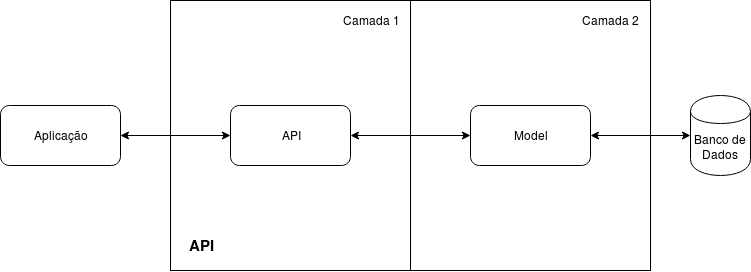
\includegraphics[scale=0.5]{figuras/software/8-api-arquitetura.png}
	\caption{Arquitetura da API}
\end{figure}

Além disso, a camada de API deverá respeitar o padrão REST quando possível, que consiste no reuso de URL endereçáveis, mudando-se o método utilizado na requisição. Quando não for possível respeitar o padrão REST, deve-se utilizar o protocolo RPC, que consiste em requisições que não necessariamente consistem no reuso de uma URL endereçavel.

\subsection{Visão de implantação}
A implantação do sistema será feita de acordo com o seguinte diagrama

\begin{figure}[!ht]
	\centering
		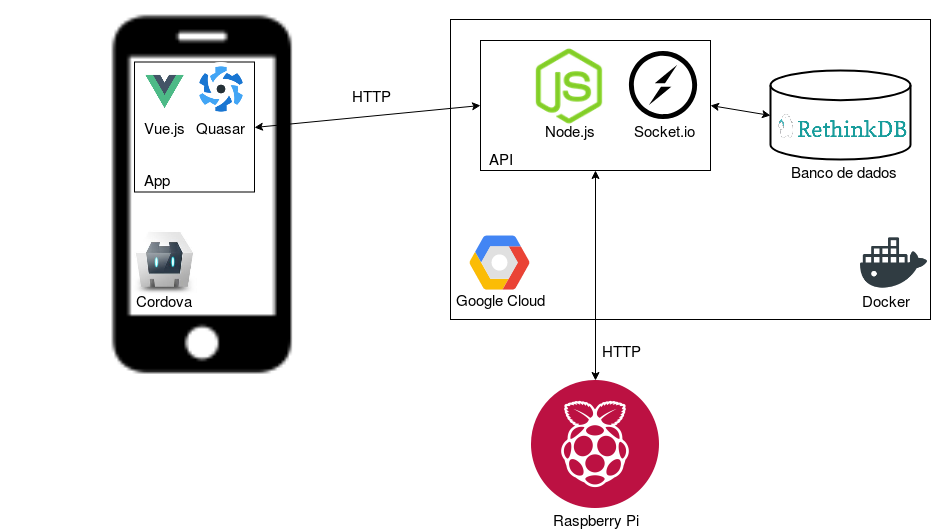
\includegraphics[scale=0.4]{figuras/software/9-implantacao.png}
	\caption{Implantação}
\end{figure}

A API, a qual diz respeito à aplicação em Node.js com a comunicação em tempo real feita pelo Socket.io, juntamente com o banco de dados, em RethinkDB, estarão disponíveis para acesso na nuvem por meio da plataforma do Google Cloud. A plataforma fará essa disponibilização através de uma imagem do Docker. A escolha do Docker foi feita para que a implantação da API independesse do serviço de nuvem utilizado. Desta forma, o Google Cloud pode ser facilmente substituído pela AWS, Microsoft Azure ou Digital Ocean, por exemplo. Sendo assim a escolha do Google Cloud foi feita apenas com base no seu período de uso gratuito sem a necessidade de vincular nenhum tipo de cartão de crédito.

O aplicativo do cliente por sua vez rodará em um celular através do Cordova. Funciona da seguinte maneira: o Quasar gera uma série de arquivos estáticos (HTML, CSS e Javascript) com base no código após desenvolvida a aplicação utilizando-se do Vue e até mesmo de componentes do próprio Quasar. O Cordova se utiliza desses arquivos estáticos para gerar uma aplicação mobile, que nada mais é do que um servidor que serve os arquivos gerados peloQuasar. Essa aplicação gerada pelo cordova se comunicará com a API na nuvem através de requisições HTTP.

Por fim, a placa Raspberry Pi que estará presente na máquina também se comunicará com
o servidor através de requisições HTTP.

\end{apendicesenv}
